% Working paper source for VeriTrace.
% Replace the document class and author block with the official AAAI author-kit
% versions before submission. The content below intentionally compiles without
% the proprietary conference style so that it can be edited and reviewed now.
\documentclass[letterpaper,twocolumn,10pt]{article}

\usepackage[margin=0.72in]{geometry}
\usepackage{amsmath,amssymb}
\usepackage{booktabs}
\usepackage{graphicx}
\usepackage{hyperref}
\usepackage{xcolor}
\usepackage{enumitem}

\hypersetup{colorlinks=true,linkcolor=blue,citecolor=blue,urlcolor=blue}
\setlist{nosep,leftmargin=*}
\newcommand{\system}{\textsc{VeriTrace}}
\newcommand{\todo}[1]{\textcolor{red}{[TODO: #1]}}

\title{From Evidence to Logic: An Interactive Neuro-Symbolic System for Fact Verification}
\author{Anonymous Authors\\
\texttt{\{author details withheld for review\}}}
\date{}

\begin{document}
\maketitle

\begin{abstract}
Fact-verification systems often return a verdict without exposing the decisions
behind it. \system{} is an interactive demonstration that decomposes a complex
claim into atomic claims, retrieves source sentences, and assesses how selected
evidence bears on each atom. For eligible membership, comparison, counting,
and extremum questions, a local language model maps source-linked inputs to typed reasoning
programs; Python validates their premises and executes supported rules
deterministically. An evidence--inference graph connects claims, evidence,
reading context, multi-sentence inferences, and resolved symbolic results before
composition-aware aggregation produces a four-way verdict. A curated recorded
walkthrough provides a network-independent conference fallback.
\end{abstract}

\section{Motivation}

Fact-verification demonstrations face two competing requirements: they must
handle natural-language evidence, yet they must also make their intermediate
decisions inspectable. \system{} addresses this tension with a deliberately
modular pipeline:
\begin{equation}
\begin{split}
C,\mathcal{D} \rightarrow \mathcal{A} \rightarrow \mathcal{E}
\rightarrow \mathcal{R} \rightarrow \mathcal{P} \rightarrow V,
\end{split}
\label{eq:pipeline}
\end{equation}
where $C$ is the input claim, $\mathcal{D}$ is a collection of source
documents, $\mathcal{A}$ contains atomic claims, $\mathcal{E}$ contains
retrieved sentences, $\mathcal{R}$ contains assessed evidence relations,
$\mathcal{P}$ contains validated symbolic results, and
$V\in\{\textsc{Supported},\textsc{Refuted},\textsc{NEI},\textsc{Conflicting}\}$.

The graph is a selected-atom overview of these artifacts, not a separate
learned predictor. Detailed programs remain in the Symbolic Checks panel, while
the graph shows only decisive assessed relations and resolved rule results.
Dataset reference labels are displayed as metadata but never enter inference.

\section{System Architecture}

\subsection{Claim Decomposition}

Qwen2.5, served locally through Ollama, rewrites $C$ into atoms
$\mathcal{A}=\{a_1,\ldots,a_m\}$. Each rewritten atom retains a verbatim source
span $g_i$ and offsets $(s_i,e_i)$ satisfying
\begin{equation}
g_i = C[s_i:e_i].
\label{eq:grounding}
\end{equation}
This constraint distinguishes the rewritten proposition from the text that
licensed it and prevents an ungrounded atom from silently entering the
pipeline. The interface also exposes a collapsed, verdict-neutral claim
structure panel based on heuristic spaCy parsing.

\subsection{Candidate Evidence Retrieval}

Documents are segmented into exact-offset sentences with PySBD. BGE-small
encodes each atomic claim as a retrieval query and every eligible source
sentence as a passage. With $f(\cdot)$ denoting the embedding model, embeddings
are $L_2$-normalized:
\begin{equation}
\hat{q}_i=\frac{f_{q}(a_i)}{\lVert f_{q}(a_i)\rVert_2},\qquad
\hat{p}_j=\frac{f_{p}(e_j)}{\lVert f_{p}(e_j)\rVert_2}.
\end{equation}
The semantic score is cosine similarity,
\begin{equation}
s_{ij}=\hat{q}_i^{\top}\hat{p}_j.
\label{eq:retrieval}
\end{equation}
The interface exposes three retrieval methods. \textsc{Semantic} ranks by
$s_{ij}$ alone. \textsc{Lexical} ranks by exact term coverage with additional
anchors for matching names, numbers, dates, and list entries. The default
\textsc{Hybrid} method combines their ranks with equal-weight reciprocal rank
fusion (RRF)~\cite{cormack-etal-2009-rrf}:
\begin{equation}
s_{\mathrm{hybrid}}(e_j)=
\frac{1}{60+r_{\mathrm{semantic}}(e_j)}+
\frac{1}{60+r_{\mathrm{lexical}}(e_j)}.
\end{equation}
Following Cormack et al., the rank constant is fixed at 60. Equal weighting
avoids introducing a collection-specific tuning parameter into the qualitative
showcase. Exact lexical score, followed by document and sentence order, breaks
otherwise equal fused scores deterministically.
The system returns up to a user-selected $k$ candidates per atom, ranked
globally, with at most three anchors from any one document when multiple
documents are present. An anchor carries at most one preceding and one following
sentence as visibly identified reading context; those neighbours do not count
toward $k$ and are not themselves highlighted as decisive evidence.

\subsection{Jurisdiction Integrity Check}

Before model assessment, a deterministic scope gate compares jurisdictions
resolved from an atom and a candidate's sentence, context, title, URL, and
document lead. Let $J_a$ and $J_e$ be the explicitly resolved jurisdiction
sets. A mismatch is declared only when both sets are non-empty and disjoint:
\begin{equation}
\operatorname{scope}(a,e)=\textsc{Mismatch}
\iff J_a\neq\varnothing \land J_e\neq\varnothing
\land J_a\cap J_e=\varnothing.
\label{eq:scope}
\end{equation}
Otherwise the result is \textsc{Match}, \textsc{Unresolved}, or
\textsc{NotApplicable}. Mismatched candidates remain visible for diagnosis but
cannot be selected as supporting or refuting evidence.

\paragraph{Example.}
Evidence from an Australian designated-organisation list cannot establish an
atom specifically about New Zealand. The scope gate excludes that candidate;
it does not treat the mismatch as a refutation and does not infer New Zealand's
position from another jurisdiction.

\subsection{Evidence Assessment}

For each atom, Qwen may select only server-owned candidate identifiers and mark
them as \textsc{Supports}, \textsc{Refutes}, or \textsc{Context}. It also
reports bundle sufficiency $u_i\in\{\textsc{Sufficient},\textsc{Partial},
\textsc{Insufficient}\}$ and missing information. If $S_i$ and $R_i$ are its
supporting and refuting selections, the decisive relations are
\begin{equation}
(S_i^{*},R_i^{*})=
\begin{cases}
(S_i,R_i), & u_i=\textsc{Sufficient},\\
(\varnothing,\varnothing), & \text{otherwise}.
\end{cases}
\label{eq:sufficiency}
\end{equation}
Selections from partial or insufficient bundles remain visible as potential
evidence but cannot enter the graph or affect the verdict. This stage is an
evidence-bundle assessment, not conventional sentence-pair NLI.

\subsection{Typed Symbolic Checks}

The symbolic layer follows the program-guided separation between reasoning-
program generation and execution advocated by ProgramFC
\cite{pan-etal-2023-fact}. Local extractors first construct typed operands and
source premise IDs. Qwen may map those grounded inputs to a program
\begin{equation}
p=(o, I, x),
\end{equation}
where $o$ is an operator, $I$ is a list of server-owned premise IDs, and $x$
contains typed operands. Qwen cannot supply the calculated result. Python
computes
\begin{equation}
\operatorname{Exec}(p)=
\begin{cases}
o(x), & \operatorname{Validate}(I,x)=\top,\\
\textsc{Unresolved}, & \text{otherwise}.
\end{cases}
\label{eq:execution}
\end{equation}

Version 1 supports six conservative operator families:
\begin{itemize}
  \item \textbf{Set membership.} Presence can establish membership. Absence
  establishes non-membership only when the cited source explicitly certifies
  that the list is exhaustive:
  \begin{equation}
  x\notin L \land \operatorname{Complete}(L)
  \Rightarrow \neg\operatorname{Member}(x,L).
  \end{equation}
  \item \textbf{Numeric comparison.} Decimal comparisons support equality and
  $<,\leq,>,\geq$ only when entity, measure, time, and units align.
  \item \textbf{Temporal comparison.} Dates are represented as intervals.
  ``Before'' is resolved only when $\max(I_1)<\min(I_2)$; overlapping or
  underspecified intervals remain unresolved.
  \item \textbf{Attribute comparison.} Explicit source attributes are tested
  for equality or inequality only after subject and attribute alignment.
  \item \textbf{Distinct-value counting.} Source values are normalized and
  counted without inferring equivalence between unstated categories.
  \item \textbf{Extremum counterexample.} One aligned larger value may refute
  a ``largest'' claim; support requires a certified complete comparison
  universe. Values with incompatible measurement definitions remain unresolved.
\end{itemize}

\paragraph{Set-membership example.}
Suppose an atom states that organisation $x$ is not designated by country $c$.
The absence of $x$ from a retrieved list is not enough. If the source says
``the complete designated list is $\{a,b,d\}$,'' Python may derive
$x\notin\{a,b,d\}$ after exact-item and jurisdiction validation. Without a
completeness certificate, the result is \textsc{Unresolved}.

\subsection{Evidence--Inference Graph}

The visualization contains four stable tiers: case claim, atomic claims,
inferences, and evidence. A multi-sentence bundle produces an inference node
only when multiple sentences are actually combined. A resolved symbolic check
produces a node containing its operator, expression, conclusion, and cited
premises. Context is collapsed inside its evidence node by default. This design
is motivated by CHECKWHY's explicit evidence-to-inference structures
\cite{si-etal-2024-checkwhy}, but \system{} does not claim CHECKWHY-style causal
verification or formal argumentation semantics.

The graph is a filtered view of the preceding stages, not an additional
selection model. It displays (i) supporting or refuting evidence selected by
Qwen only when the corresponding bundle is sufficient and the relation is
accepted by deterministic aggregation, and (ii) the cited premises of symbolic
programs that Python resolves as proved or disproved. Retrieved but unselected
candidates, reading context, provisional relations, jurisdiction mismatches,
and unresolved or inapplicable symbolic checks remain available in their
inspection panels but are omitted from the default graph.

\begin{figure}[t]
  \centering
  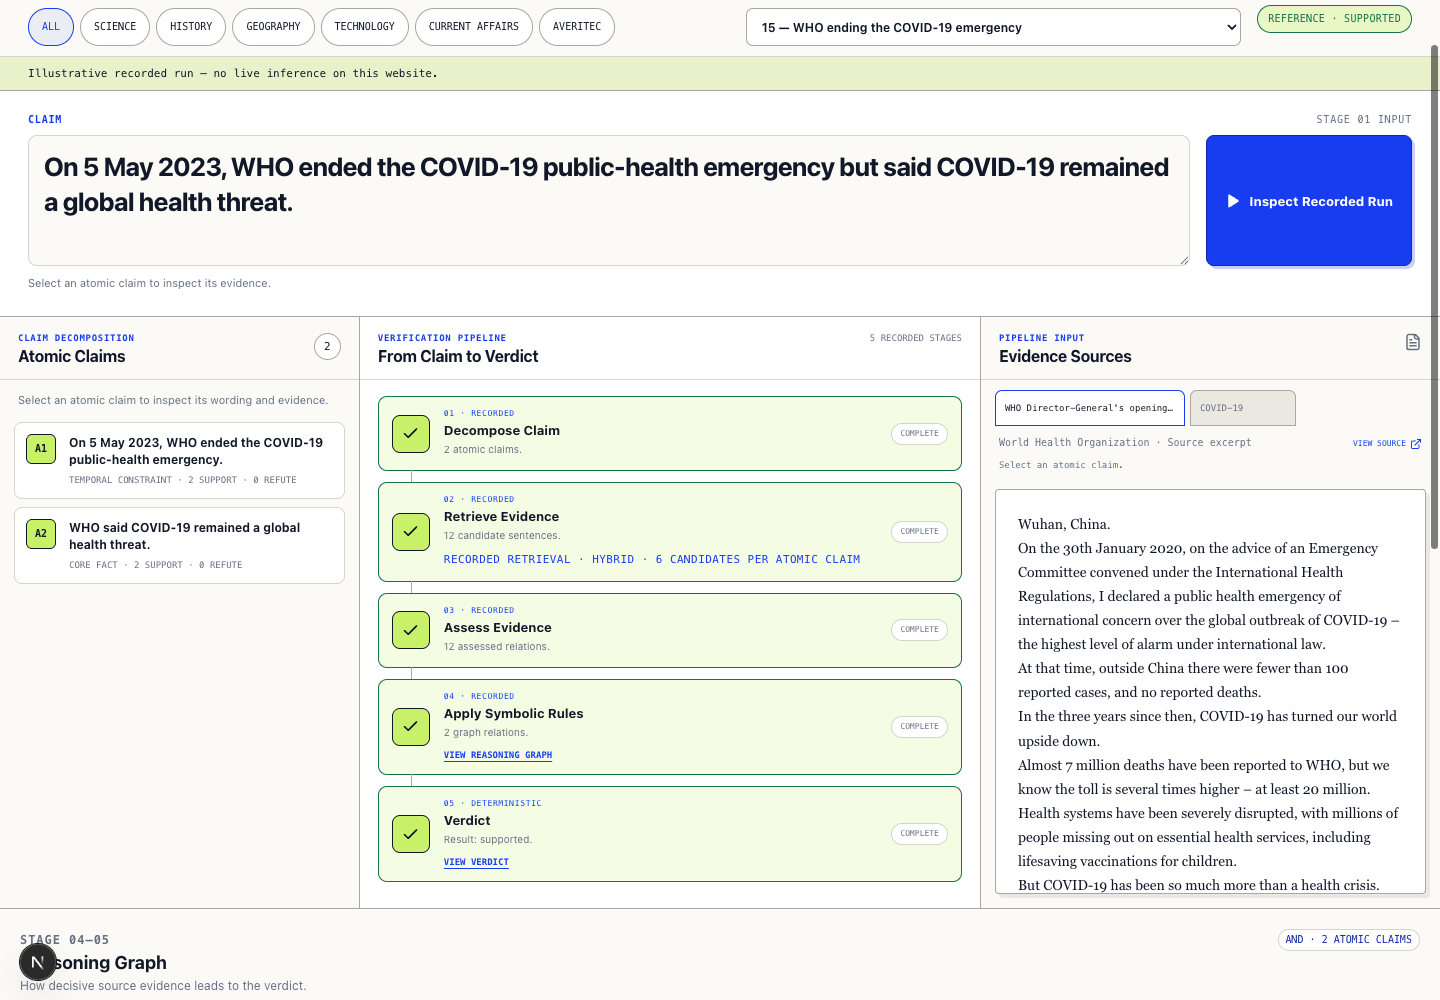
\includegraphics[width=\linewidth]{screenshots/veritrace-desktop.png}
  \caption{The recorded walkthrough with claim decomposition, the five-stage
  pipeline, selected-atom inspection, and source-grounded evidence. The
  reference label is displayed separately from the computed verdict.}
  \label{fig:interface}
\end{figure}

\begin{figure}[t]
  \centering
  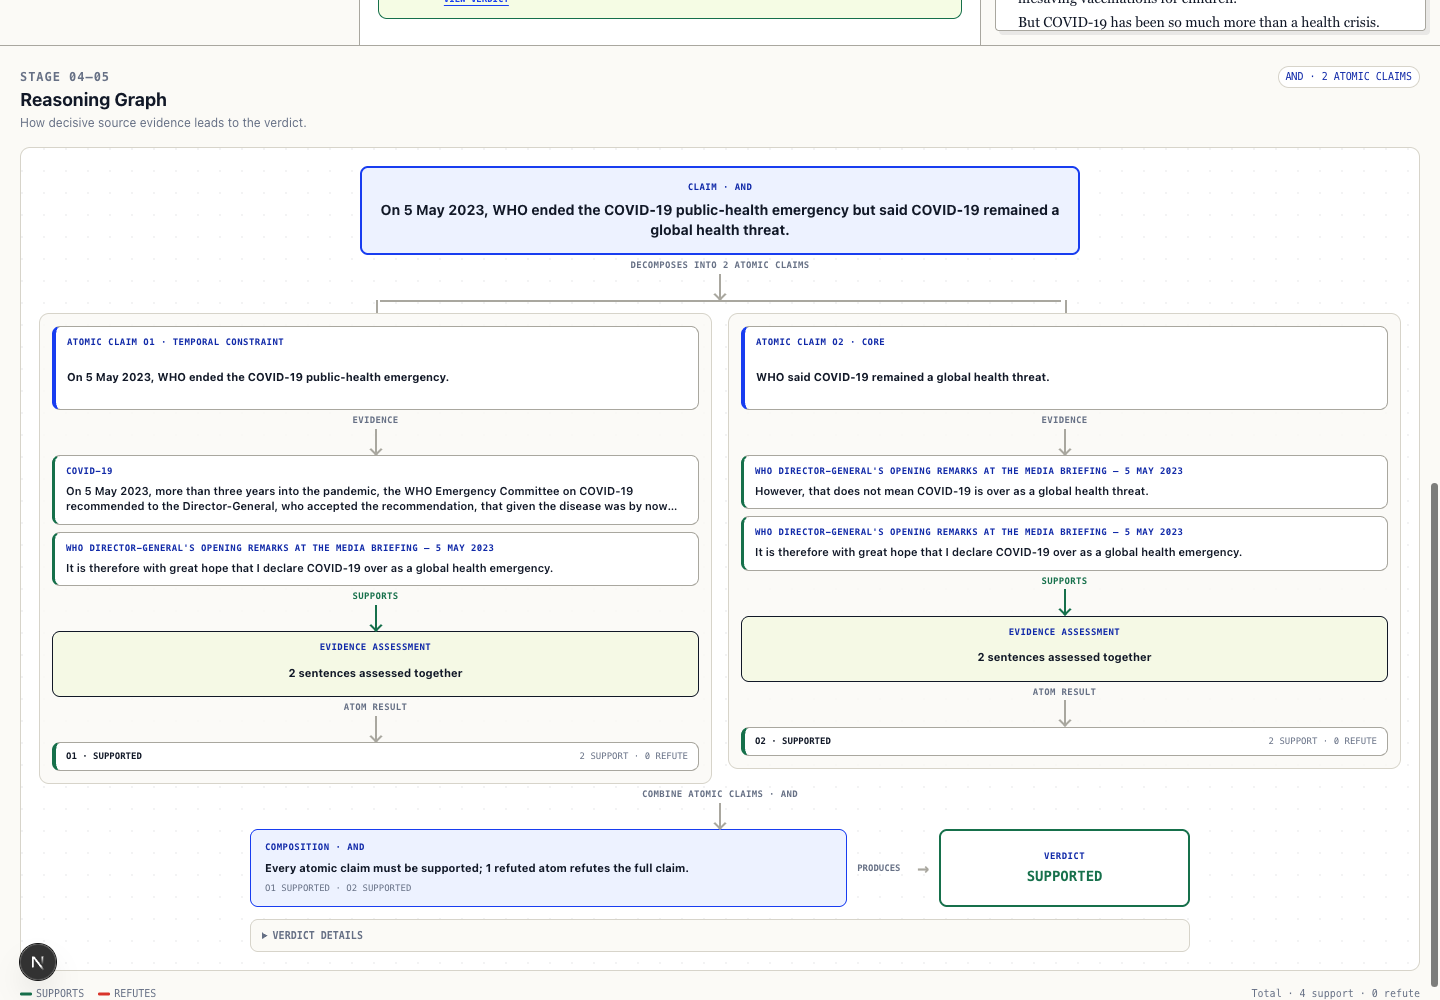
\includegraphics[width=\linewidth]{screenshots/veritrace-graph.png}
  \caption{Selected-atom reasoning graph. A Python-executed symbolic result
  cites its source premise, while unrelated atomic claims are visually
  subordinate.}
  \label{fig:graph}
\end{figure}

\subsection{Composition-Aware Verdict}

Each atom receives an evidence state from its decisive assessed relations and
resolved symbolic derivations:
\begin{equation}
z_i=
\begin{cases}
\textsc{Conflicting}, & S_i^{*}\neq\varnothing\land R_i^{*}\neq\varnothing,\\
\textsc{Supported}, & S_i^{*}\neq\varnothing\land R_i^{*}=\varnothing,\\
\textsc{Refuted}, & S_i^{*}=\varnothing\land R_i^{*}\neq\varnothing,\\
\textsc{NEI}, & \text{otherwise}.
\end{cases}
\label{eq:atomstate}
\end{equation}
Resolved Python results are added to the corresponding support or refutation
set before Eq.~\ref{eq:atomstate}. For conjunctive claims,
\begin{equation}
V_{\land}=\begin{cases}
\textsc{Refuted}, & \exists i:z_i=\textsc{Refuted},\\
\textsc{Conflicting}, & \nexists i:z_i=\textsc{Refuted}\land
  \exists i:z_i=\textsc{Conflicting},\\
\textsc{Supported}, & \forall i:z_i=\textsc{Supported},\\
\textsc{NEI}, & \text{otherwise}.
\end{cases}
\label{eq:and}
\end{equation}
For disjunctive claims, support is established by any supported atom, while
refutation requires every atom to be refuted; otherwise conflicting and
insufficient cases are handled conservatively. A separately grounded material-
omission certificate may produce \textsc{Conflicting} only when it cites
decisive, sufficient evidence.

\section{Interactive Demonstration}

The interface exposes each stage without requiring visitors to understand the
implementation stack. A typical interaction is:
\begin{enumerate}
  \item Choose a topic and select a source-grounded example or AVeriTeC case,
  or enter a custom claim and sources.
  \item Decompose the claim and inspect exact grounding spans.
  \item Select an atom to inspect candidate evidence across source tabs.
  \item Review scope exclusions, sufficiency, and assessed relations.
  \item Inspect any Python-executed symbolic result and its premises.
  \item Follow the displayed graph to the deterministic verdict.
\end{enumerate}
The complete pipeline runs locally. The hosted Vercel site presents recorded
runs and states that no live inference occurs there.

The interface makes the neural--symbolic boundary explicit: Qwen maps grounded
inputs to a typed rule, Python validates the cited premises and executes the
rule, and deterministic composition produces the verdict. Unresolved checks
remain inspectable but do not enter the graph or aggregation.

\begin{figure}[t]
  \centering
  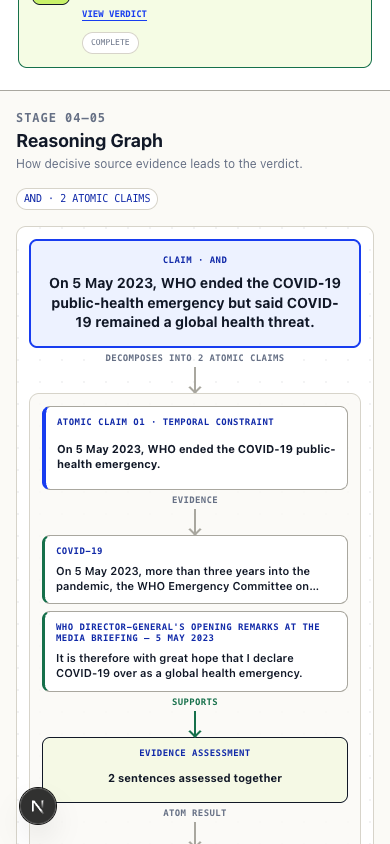
\includegraphics[width=0.62\linewidth]{screenshots/veritrace-mobile.png}
  \caption{Mobile selected-atom view. Evidence Assessment precedes the
  inspectable Symbolic Checks panel; Claim Structure remains secondary.}
  \label{fig:atom}
\end{figure}

\section{Source-Grounded Showcase}

The hosted walkthrough contains 18 qualitative cases: 15 constructed claims
across Science, History, Geography, Technology, and Current Affairs, plus six
curated AVeriTeC cases retained for realism. Each constructed case contains two
contiguous 150--400-word excerpts from distinct authoritative sources. Claims
and intended interpretations are authored, but source passages are stored
verbatim after extraction rather than paraphrased or converted into evidence
cards. Publisher, canonical URL, retrieval date, extraction offsets, and hashes
are audited offline. Reference labels remain display-only metadata and are
withheld from inference. This collection demonstrates contrasting reasoning
paths; it is not an accuracy benchmark.

\begin{table}[t]
\centering
\scriptsize
\caption{Representative showcase interactions.}
\label{tab:showcases}
\begin{tabular}{p{0.23\linewidth}p{0.69\linewidth}}
\toprule
Case & Demonstrated behaviour\\
\midrule
Einstein's Nobel citation & Attribute inequality between relativity and the
grounded prize reason.\\
Curie's Nobel fields & Distinct-value counting across two sources.\\
Canberra population & An aligned larger value refutes a superlative.\\
Everest and Mauna Kea & Incompatible measurement definitions force an
unresolved symbolic result.\\
Finland and Sweden & Before/after execution over two accession dates.\\
UN Security Council & Absence supports non-membership only when the source
certifies the complete permanent-member list.\\
\bottomrule
\end{tabular}
\end{table}

The walkthrough does not present a resolved symbolic result unless its source,
measure, and typed operands align. Cases with superficially plausible but
semantically mismatched premises are excluded from the showcase rather than
used to produce a more attractive graph.

Six AVeriTeC cases complement the constructed examples: development cases 15,
142, 146, 392, 413, and 435. They use recovered source documents only. The
public selector gives every case equal visual weight; category and origin groups
support navigation without implying that one example is more valid than another.

\paragraph{Demonstration validation before submission.}
\begin{itemize}
  \item \todo{Approve the tracked atom, operator, verdict, and premise audit for
  all 18 recorded runs.}
  \item \todo{Confirm that every default selected-atom graph contains no more
  than nine visible nodes at the presentation display resolution.}
  \item \todo{Record hardware details and rehearse both the live and offline
  walkthrough paths.}
\end{itemize}

\section{Limitations and Responsible Use}

\system{} verifies claims against supplied documents; it does not establish
source authority or perform open-web fact checking. Its jurisdiction resolver
is conservative but cannot disambiguate every geographic mention. The symbolic
operators do not cover fuzzy entity linking, unstated arithmetic, unit
conversion, relative time, causal rules, or general natural logic. A resolved
rule result is valid only for its displayed premises and supported operator.
Qwen assessments can still be wrong, and no accuracy improvement from symbolic
execution is claimed. The hosted site
uses immutable recorded runs; live local inference requires the packaged BGE
weights, spaCy model, and Ollama/Qwen configuration.

\section{Conclusion}

\system{} demonstrates a compact path from natural-language evidence to
inspectable, source-bound computation. Neural components decompose claims,
retrieve candidates, and assess evidence; deterministic checks enforce source
scope, validate symbolic premises, execute supported operators, and aggregate
the displayed relations. The system's contribution is not a general-purpose
logic engine, but an interactive architecture in which visitors can inspect
where model judgment ends and deterministic reasoning begins.

\bibliographystyle{plain}
\bibliography{references}

\end{document}
